\documentclass[12pt]{article}

\usepackage{sbc-template}
\usepackage{graphicx,url}
\usepackage[utf8]{inputenc}
\usepackage[T1]{fontenc}
\usepackage[brazil]{babel}
\usepackage{amsmath,amssymb}
\usepackage{booktabs}
\usepackage{pgfplots}
\usetikzlibrary{arrows.meta,positioning}

\pgfplotsset{compat=1.18}

% Figuras empacotadas com este documento.
\graphicspath{{figuras/}}

\sloppy

% ============================================================
% REFERENCIAS BIBLIOGRAFICAS
% ============================================================

\begin{filecontents*}{referencias_grafos.bib}

@article{felzenszwalb2004,
  author = {Felzenszwalb, Pedro F. and
            Huttenlocher, Daniel P.},
  title = {Efficient Graph-Based Image Segmentation},
  journal = {International Journal of Computer Vision},
  volume = {59},
  number = {2},
  pages = {167--181},
  year = {2004}
}

@article{rand1971,
  author = {Rand, William M.},
  title = {Objective Criteria for the Evaluation
           of Clustering Methods},
  journal = {Journal of the American Statistical Association},
  volume = {66},
  number = {336},
  pages = {846--850},
  year = {1971}
}

@article{meila2007,
  author = {Meila, Marina},
  title = {Comparing Clusterings---An Information
           Based Distance},
  journal = {Journal of Multivariate Analysis},
  volume = {98},
  number = {5},
  pages = {873--895},
  year = {2007}
}

@article{tarjan1975,
  author = {Tarjan, Robert Endre},
  title = {Efficiency of a Good But Not Linear
           Set Union Algorithm},
  journal = {Journal of the ACM},
  volume = {22},
  number = {2},
  pages = {215--225},
  year = {1975}
}

@book{cormen2022,
  author = {Cormen, Thomas H. and Leiserson, Charles E.
            and Rivest, Ronald L. and Stein, Clifford},
  title = {Introduction to Algorithms},
  edition = {4},
  publisher = {MIT Press},
  year = {2022}
}

@misc{repositorio2026,
  author = {{Equipe de Desenvolvimento}},
  title = {Segmentação Hierárquica de Imagens com Grafos},
  year = {2026},
  howpublished = {\url{https://github.com/RafaelLopes1810/grafos-segmentacao-hierarquica}},
  note = {Código-fonte e resultados experimentais}
}

\end{filecontents*}

% ============================================================
% TITULO E AUTORES
% ============================================================

\title{
Segmentação Hierárquica de Imagens Baseada em Grafos:
Implementação e Avaliação Experimental
}

\author{
Ana Luiza Rezende\inst{1},
Gustavo Costa Gabrich\inst{1},\\
Otto Esteves Oliveira\inst{1},
Rafael de Oliveira Caldeira Lopes\inst{1}
}

\address{
Pontifícia Universidade Católica de Minas Gerais
(PUC Minas)\\
Belo Horizonte -- MG -- Brasil
}

\begin{document}

\maketitle

% ============================================================
% ABSTRACT
% ============================================================

\begin{abstract}
This paper presents a graph-based hierarchical image
segmentation system. Pixels are modeled as vertices connected
by weighted edges, and initial regions are obtained using
the Felzenszwalb--Huttenlocher method and a custom Union-Find
implementation. Successive region merges generate nested
partitions and region adjacency graphs. The application
integrates a Python/FastAPI backend and a React frontend.
Evaluation includes mathematical invariants, automated tests,
color homogeneity and performance measurements.
Five runs per resolution resulted in mean processing times
of 474.31, 1471.35 and 3257.31 milliseconds for maximum
image dimensions of 160, 320 and 480 pixels, respectively.
\end{abstract}

% ============================================================
% RESUMO
% ============================================================

\begin{resumo}
Este trabalho apresenta um sistema de segmentação hierárquica
de imagens baseado em grafos. Os pixels são representados
por vértices conectados por arestas ponderadas pela diferença
de cores. A segmentação inicial utiliza o método de
Felzenszwalb--Huttenlocher e uma implementação própria de
Union-Find. Fusões sucessivas produzem partições aninhadas
e grafos de adjacência de regiões. A aplicação integra
Python, FastAPI e React. A avaliação inclui validação
matemática, testes automatizados, homogeneidade de cores
e análise de desempenho. Em cinco execuções por resolução,
os tempos médios foram 474,31 ms, 1.471,35 ms e
3.257,31 ms para dimensões máximas de 160, 320 e
480 pixels, respectivamente.
\end{resumo}

% ============================================================
\section{Introdução}
\label{sec:introducao}
% ============================================================

A segmentação de imagens é uma tarefa da visão computacional
que busca dividir uma imagem em regiões de características
semelhantes. Essas regiões podem auxiliar na análise de
objetos, na interpretação de cenas e em outras aplicações
que exigem organização de informações visuais.

Uma das abordagens existentes consiste em representar a
imagem como um grafo ponderado. Nessa estrutura, cada pixel
corresponde a um vértice, enquanto as relações de vizinhança
são representadas por arestas. Os pesos indicam a diferença
entre as características dos pixels conectados.

O método de Felzenszwalb e Huttenlocher
\cite{felzenszwalb2004} utiliza essa representação
para agrupar componentes considerando diferenças internas
e relações entre regiões. Entretanto, uma única segmentação
nem sempre apresenta o nível de detalhamento adequado
para todas as análises.

A segmentação hierárquica permite observar diferentes
partições da mesma imagem, desde regiões pequenas até
agrupamentos maiores, preservando uma relação de inclusão
entre os níveis.

O objetivo deste trabalho é implementar e avaliar uma
ferramenta de segmentação hierárquica baseada em grafos,
com estruturas de dados e algoritmos próprios, interface
gráfica e análise experimental reproduzível.

As principais funcionalidades desenvolvidas são a
construção do grafo de pixels, a segmentação inicial,
a formação da hierarquia, a geração dos grafos de
adjacência de regiões (RAGs) e a visualização interativa
dos resultados.

A avaliação compreende testes automatizados, verificação
de propriedades matemáticas, métricas de segmentação
e medições de desempenho em diferentes resoluções.

% ============================================================
\section{Fundamentação Teórica}
\label{sec:fundamentacao}
% ============================================================

\subsection{Representação de imagens por grafos}

Um grafo ponderado é definido por:

\begin{equation}
G=(V,E,w),
\end{equation}

em que $V$ é o conjunto de vértices, $E$ o conjunto
de arestas e $w$ uma função que associa pesos às arestas.

Para uma imagem com largura $W$ e altura $H$, existem
$N=W\cdot H$ pixels. Cada pixel é representado por
um vértice, enquanto as arestas conectam pixels vizinhos.

O sistema permite utilizar conectividade 4, considerando
vizinhos horizontais e verticais, ou conectividade 8,
incluindo as diagonais.

Os pesos representam a dissimilaridade entre pixels.
No espaço RGB, utiliza-se a distância euclidiana entre
seus três canais de cor.

\subsection{Segmentação e Union-Find}

A segmentação inicial utiliza o algoritmo de
Felzenszwalb--Huttenlocher \cite{felzenszwalb2004}.
O procedimento processa as arestas em ordem crescente
de peso e avalia a união entre componentes distintas.

A estrutura Union-Find mantém os conjuntos de pixels
agrupados e oferece as operações \texttt{find},
para identificar o representante de uma componente,
e \texttt{union}, para combinar componentes.

A implementação utiliza compressão de caminho e
união por posto, técnicas associadas à eficiência
das operações sobre conjuntos disjuntos
\cite{tarjan1975,cormen2022}.

\subsection{Hierarquia e grafo de regiões}

Após a segmentação inicial, o sistema realiza fusões
sucessivas entre regiões adjacentes, formando uma
estrutura hierárquica semelhante a um dendrograma.

Os níveis da hierarquia representam partições com
diferentes quantidades de regiões. Cada região de
um nível detalhado deve estar inteiramente contida
em alguma região de um nível mais agregado.

Para representar as relações espaciais entre essas
regiões, utiliza-se um grafo de adjacência (RAG).
Nesse grafo, cada vértice corresponde a uma região
e as arestas indicam fronteiras compartilhadas.

% ============================================================
\section{Modelagem Matemática}
\label{sec:modelagem}
% ============================================================

\subsection{Construção do grafo de pixels}

Considere uma imagem RGB e dois pixels vizinhos
$p$ e $q$, com valores de cor
$(R_p,G_p,B_p)$ e $(R_q,G_q,B_q)$.

O peso da aresta que os conecta é calculado por:

\begin{equation}
w(p,q)=\sqrt{
(R_p-R_q)^2+
(G_p-G_q)^2+
(B_p-B_q)^2
}.
\label{eq:pesos}
\end{equation}

O sistema também permite calcular dissimilaridades
no espaço de cores CIELAB, além de aplicar suavização
gaussiana antes da construção do grafo.

\subsection{Critério de agrupamento}

Sejam $C_1$ e $C_2$ duas componentes distintas.
O algoritmo considera o peso da aresta analisada,
a diferença interna $Int(C)$ e um parâmetro $k$.

As componentes são unidas quando:

\begin{equation}
w(e)\leq
\min\left\{
Int(C_1)+\frac{k}{|C_1|},
Int(C_2)+\frac{k}{|C_2|}
\right\}.
\label{eq:criterio}
\end{equation}

O parâmetro $k$ controla a escala do agrupamento,
enquanto $|C|$ corresponde ao número de pixels
da componente.

Após a primeira passagem, componentes menores
que o parâmetro \texttt{min\_size} podem ser
agrupadas a componentes vizinhas.

\subsection{Partições hierárquicas}

Uma segmentação é uma partição
$\mathcal{P}=\{C_1,\ldots,C_R\}$ do conjunto
de pixels $\Omega$, satisfazendo:

\begin{equation}
\bigcup_{i=1}^{R} C_i=\Omega
\quad\text{e}\quad
C_i\cap C_j=\varnothing,\;i\neq j.
\end{equation}

A construção hierárquica parte de uma segmentação
inicial com $R$ regiões. Cada fusão substitui
duas regiões disjuntas $A$ e $B$ pela união
$A\cup B$.

Após $t$ fusões:

\begin{equation}
|\mathcal{P}_t|=R-t.
\end{equation}

Como nenhuma fusão redistribui pixels entre
regiões não relacionadas, as partições permanecem
aninhadas:

\begin{equation}
\forall A\in\mathcal{P}_t,\;
\exists B\in\mathcal{P}_{t+1}
\text{ tal que } A\subseteq B.
\label{eq:aninhamento}
\end{equation}

Uma sequência completa de $R-1$ fusões produz
uma única região e uma árvore binária com
$2R-1$ nós.

A cor média da união de duas regiões é obtida
pela média ponderada de suas áreas:

\begin{equation}
\mu_{A\cup B}=
\frac{|A|\mu_A+|B|\mu_B}{|A|+|B|}.
\label{eq:media}
\end{equation}

\subsection{Seleção dos níveis hierárquicos}

A implementação utiliza \texttt{HierarchyTree} para registrar cada fusão
em um nó interno com referências para seus dois filhos. Os nós-folha
correspondem às regiões produzidas pela segmentação inicial. O histórico
de fusões permite reconstruir cortes por número de regiões ou por limiar
de altura, sem executar novamente a segmentação de pixels.

Quando a cor média é recalculada após uma fusão, a distância usada para
escolher a próxima fusão não precisa ser numericamente crescente.
Por isso, a altura de um nó interno é definida como o máximo entre
o peso de sua fusão e as alturas de seus filhos:

\begin{equation}
h(v)=\max\{w(v),h(v_{\mathrm{esq}}),h(v_{\mathrm{dir}})\}.
\label{eq:altura}
\end{equation}

Assim, a altura do pai não é inferior à dos descendentes, o que mantém
a consistência dos cortes por limiar. Nos cortes por quantidade,
o sistema aplica um prefixo do histórico e obtém exatamente a
cardinalidade solicitada. Para uma partição inicial com pelo menos
duas regiões, a interface normalmente apresenta até oito níveis,
terminando com duas regiões; a árvore interna registra também
a fusão final que produz uma única região.

\subsection{Validação da homogeneidade}

A homogeneidade é avaliada pelo erro quadrático
médio de cores, denominado MSE.

Para cada região $C$, seja $\mu_C$ a média RGB
exata de seus pixels. Define-se:

\begin{equation}
MSE(\mathcal{P})=
\frac{1}{3N}
\sum_{C\in\mathcal{P}}
\sum_{p\in C}
\|x_p-\mu_C\|^2,
\label{eq:mse}
\end{equation}

em que $N$ é o número de pixels da imagem.

Valores menores indicam maior uniformidade
das cores dentro das regiões.

A fusão de duas regiões apresenta a seguinte
identidade de soma de erros quadráticos:

\begin{equation}
\begin{split}
&SSE(A\cup B)-SSE(A)-SSE(B)\\
&=\frac{|A||B|}{|A|+|B|}
\|\mu_A-\mu_B\|^2\geq 0.
\end{split}
\label{eq:sse}
\end{equation}

Portanto, quando regiões são agregadas em uma
mesma imagem, o MSE não pode diminuir:

\begin{equation}
MSE(\mathcal{P}_{t+1})
\geq MSE(\mathcal{P}_t).
\label{eq:monotonicidade}
\end{equation}

Essa propriedade fundamenta os testes de
validação matemática da hierarquia.
A igualdade ocorre quando as regiões fundidas
possuem a mesma cor média.

\subsection{Métricas de comparação}

O projeto também implementa Rand Index (RI)
e Variation of Information (VI).

O RI mede a concordância entre pares de pixels
nas partições comparadas \cite{rand1971}:

\begin{equation}
RI=\frac{a+b}{\binom{N}{2}},
\end{equation}

em que $a$ representa os pares agrupados nas
duas partições e $b$ os pares separados em ambas.

A VI utiliza conceitos de entropia e informação
mútua para avaliar a diferença entre
agrupamentos \cite{meila2007}:

\begin{equation}
VI(P,Q)=H(P)+H(Q)-2I(P;Q).
\end{equation}

Na ausência de uma segmentação de referência,
essas métricas avaliam a concordância entre
partições, não a qualidade semântica dos objetos
identificados.

% ============================================================
\section{Arquitetura e Implementação}
\label{sec:arquitetura}
% ============================================================

\subsection{Organização do sistema}

O sistema utiliza uma arquitetura composta por
backend Python/FastAPI e frontend React/Vite.

O backend implementa a leitura de imagens,
construção dos grafos, segmentação, hierarquia
e avaliação das regiões.

O frontend permite carregar imagens, configurar
parâmetros, selecionar níveis hierárquicos
e visualizar as segmentações e seus RAGs.

A Figura~\ref{fig:componentes} apresenta
os principais componentes da aplicação.

\begin{figure}[htbp]
\centering
\begin{tikzpicture}[
>=Latex,
node distance=2.5mm,
modulo/.style={draw=black!45, rounded corners=2.5pt,
minimum width=2.18cm, minimum height=1.35cm,
align=center, font=\scriptsize, text width=1.95cm,
inner sep=2pt},
seta/.style={-Latex,thick,draw=black!65}
]
\node[modulo,fill=blue!11] (front) {\textbf{Frontend}\\React + Vite\\\texttt{App.jsx}};
\node[modulo,fill=violet!12,right=3mm of front] (api) {\textbf{API REST}\\FastAPI\\\texttt{main.py}};
\node[modulo,fill=blue!6,right=3mm of api] (grafo) {\textbf{Grafo}\\Imagem RGB\\Pixels e arestas};
\node[modulo,fill=orange!10,right=3mm of grafo] (seg) {\textbf{Segmentação}\\Felzenszwalb\\Union-Find};
\node[modulo,fill=green!11,right=3mm of seg] (hier) {\textbf{Hierarquia}\\Fusões\\RAG};
\node[modulo,fill=yellow!15,right=3mm of hier] (met) {\textbf{Avaliação}\\MSE\\RI / VI};
\draw[seta] (front) -- (api);
\draw[seta] (api) -- (grafo);
\draw[seta] (grafo) -- (seg);
\draw[seta] (seg) -- (hier);
\draw[seta] (hier) -- (met);
\end{tikzpicture}
\caption{Arquitetura lógica e componentes principais do sistema.
A API coordena os módulos Python; as setas indicam o fluxo de processamento.}
\label{fig:componentes}
\end{figure}

\subsection{Estruturas e módulos}

A classe \texttt{Graph}, implementada em
\path{core/graph.py}, representa grafos ponderados
não direcionados por listas de adjacência.

A classe \texttt{UnionFind}, em
\path{core/union_find.py}, mantém as componentes
e seus atributos auxiliares.

O módulo \texttt{imaging} realiza a leitura,
o redimensionamento e a construção do grafo
de pixels.

A segmentação inicial está implementada em
\path{segmentation/felzenszwalb.py}.

As classes \texttt{HierarchyTree},
\texttt{HierarchyNode} e \texttt{HierarchyLevel}
representam o histórico das fusões e os cortes
hierárquicos.

O módulo \path{region_graph.py} constrói
os RAGs e calcula os atributos das regiões.

O diagrama de classes é apresentado
na Figura~\ref{fig:classes}.

\begin{figure}[htbp]
\centering
\begin{tikzpicture}[
>=Latex,
classe/.style={draw=black!50,rounded corners=2pt,
minimum width=4.25cm,minimum height=1.8cm,
text width=3.95cm,align=left,inner sep=4pt,
font=\footnotesize},
rel/.style={-Latex,thin,draw=black!60}
]
\node[classe,fill=blue!8] (graph) at (0,0) {\textbf{Graph}\\\scriptsize Lista de adjacência;\\\scriptsize vértices e arestas};
\node[classe,fill=blue!8] (uf) at (5.0,0) {\textbf{UnionFind}\\\scriptsize \texttt{find}, \texttt{union};\\\scriptsize tamanho e peso interno};
\node[classe,fill=green!8] (region) at (10,0) {\textbf{Region}\\\scriptsize Área, cor média,\\\scriptsize centroide, caixa};
\node[classe,fill=green!8] (rag) at (0,-2.55) {\textbf{RegionGraph}\\\scriptsize Grafo de regiões;\\\scriptsize rótulos e atributos};
\node[classe,fill=violet!9] (node) at (5,-2.55) {\textbf{HierarchyNode}\\\scriptsize Filhos, pai, peso\\\scriptsize e altura da fusão};
\node[classe,fill=violet!9] (tree) at (10,-2.55) {\textbf{HierarchyTree}\\\scriptsize Histórico de fusões;\\\scriptsize cortes e níveis};
\draw[rel] (rag.north) -- (graph.south);
\draw[rel] (tree.north) -- (region.south);
\draw[rel] (tree.west) -- (node.east);
\draw[rel,dashed] (tree.north west) -- (uf.south east);
\end{tikzpicture}
\caption{Diagrama simplificado das principais classes e relações.
Associações contínuas indicam referências mantidas; linha tracejada indica utilização.}
\label{fig:classes}
\end{figure}

\subsection{Atributos de regiões e relações espaciais}

Cada região é representada por um identificador, sua área em pixels,
a cor RGB média, o centroide geométrico e uma caixa delimitadora.
O RAG é recalculado para cada nível a partir da matriz de rótulos.
Duas regiões são adjacentes quando ocupam pixels que compartilham
uma borda horizontal ou vertical. Essa regra de fronteira do RAG
é distinta da opção de conectividade 4 ou 8 usada no grafo inicial.

A separação entre o grafo de pixels e o grafo de regiões reduz a
complexidade da visualização. Enquanto o primeiro contém dezenas
de milhares de vértices nas resoluções avaliadas, o segundo contém
um vértice por região presente no corte selecionado. Por exemplo,
no nível inicial da imagem de 320 pixels são 186 vértices no RAG,
ao passo que no último nível são apenas dois. O frontend utiliza
centroides para posicionar os vértices e exibe arestas para
representar as adjacências entre regiões.

\subsection{API e interface gráfica}

A API disponibiliza os endpoints
\texttt{GET /health} e \texttt{POST /segment}.

O endpoint de segmentação recebe uma imagem
e os parâmetros escolhidos pelo usuário,
valida a requisição e executa o processamento.

O resultado é retornado em JSON e contém
as dimensões da imagem, estatísticas do grafo,
tempos de processamento e níveis hierárquicos.

Para cada nível, são enviados a imagem
segmentada, os identificadores das regiões,
suas adjacências e o MSE. As imagens
são transmitidas em Base64.

Na interface, o usuário pode alternar entre
os níveis já processados sem executar uma
nova requisição à API.

A Figura~\ref{fig:interface_real} registra a interface em funcionamento
com a imagem do carro. À esquerda, observa-se a comparação visual
entre a imagem de entrada e a segmentação inicial; à direita,
os gráficos exibem o número de regiões e o MSE nos níveis da
hierarquia. Os valores são atualizados ao selecionar outro nível,
sem uma nova execução da API.

\begin{figure}[htbp]
\centering
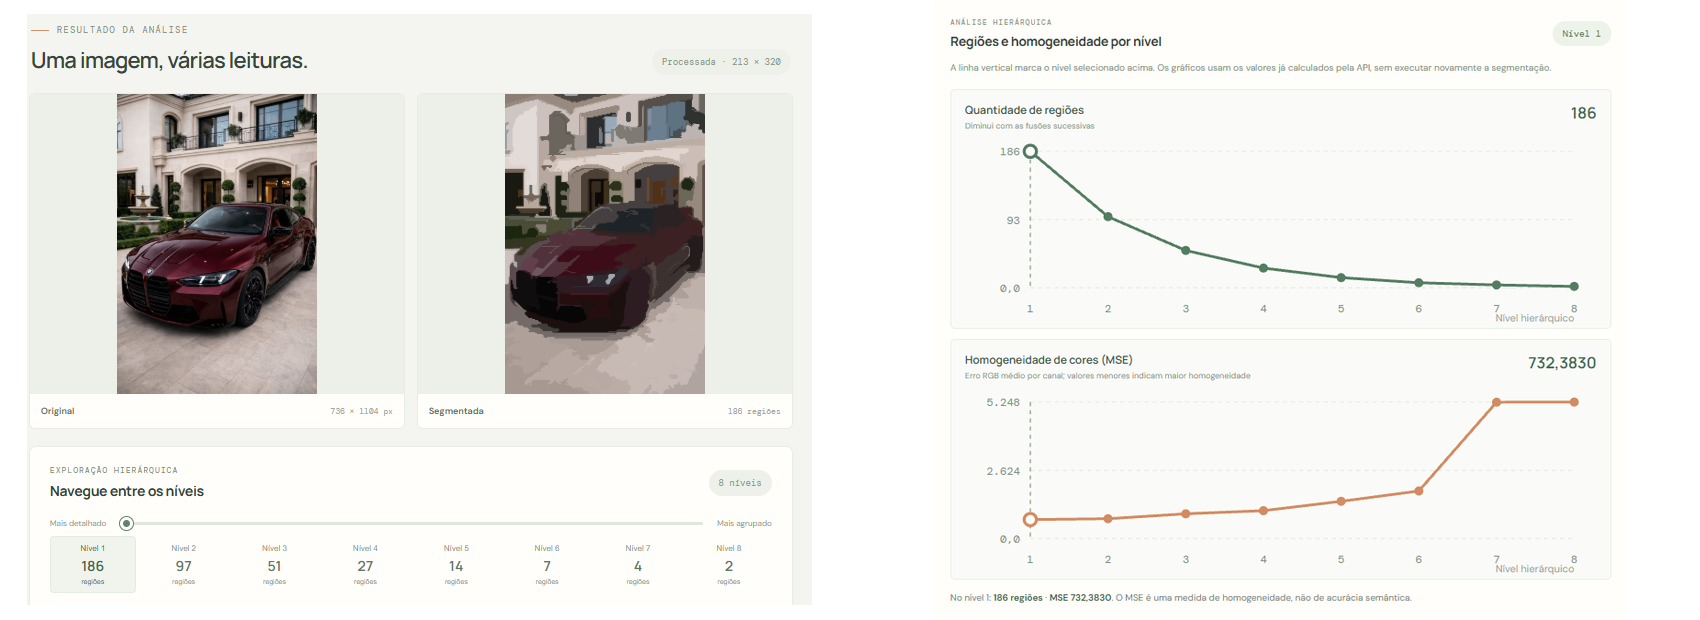
\includegraphics[
  width=.96\textwidth,
  height=5.5cm,
  keepaspectratio
]{interface_segmentacao_metricas.png}
\caption{Interface do sistema durante um teste com a imagem do
carro: comparação da segmentação e gráficos hierárquicos de regiões e MSE.}
\label{fig:interface_real}
\end{figure}

A sequência dessas operações é apresentada
na Figura~\ref{fig:sequencia}.

\begin{figure}[htbp]
\centering
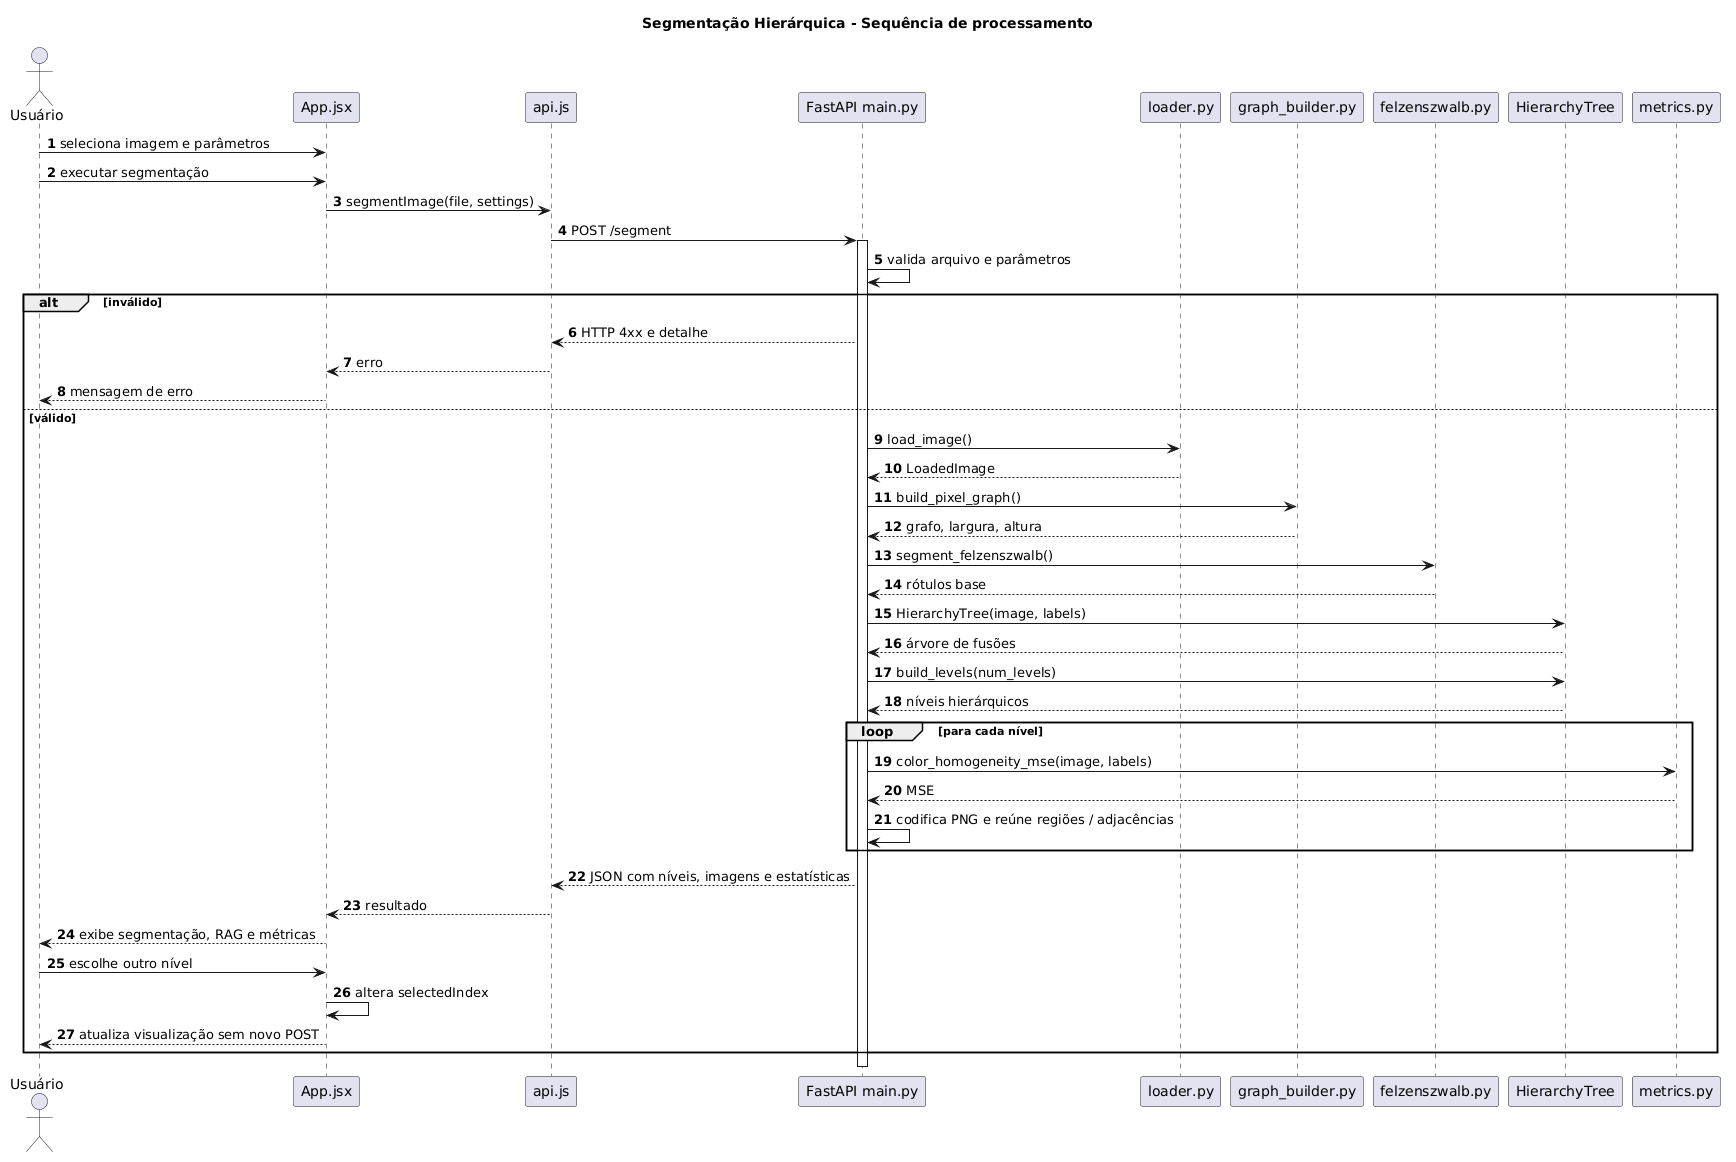
\includegraphics[
width=.97\textwidth,
height=6.0cm,
keepaspectratio
]{diagrama_sequencia.png}
\caption{Sequência principal do processamento da imagem.}
\label{fig:sequencia}
\end{figure}

\subsection{Responsabilidades e contribuições dos integrantes}

O projeto foi desenvolvido de forma colaborativa. A distribuição das
contribuições abaixo foi identificada no histórico de commits do
repositório e deve ser confirmada pelos integrantes antes da entrega.

\begin{itemize}
  \item \textbf{Rafael de Oliveira Caldeira Lopes:} implementação da
  leitura e preparação das imagens, construção do grafo de pixels,
  segmentação Felzenszwalb--Huttenlocher, hierarquia de fusões,
  grafo de adjacência de regiões (RAG) e API FastAPI, com seus testes.

  \item \textbf{Otto Esteves Oliveira:} desenvolvimento do frontend
  em React e Vite, incluindo upload, configuração dos parâmetros,
  integração com a API, comparação de imagens, navegação entre
  níveis hierárquicos e visualização do RAG.

  \item \textbf{Ana Luiza Rezende:} implementação das métricas de
  avaliação (RI, VI e MSE), integração das estatísticas à interface,
  testes adicionais e validação matemática das partições,
  benchmark reproduzível e documentação dos resultados.

  \item \textbf{Gustavo Costa Gabrich:} elaboração dos diagramas UML,
  implementação e integração dos gráficos de quantidade de regiões
  e MSE por nível e atualização dos arquivos README com instruções
  de instalação, execução e avaliação.
\end{itemize}

\subsection{Complexidade computacional}

Para uma imagem com $N$ pixels, a construção
do grafo utiliza $N$ vértices e uma quantidade
de arestas proporcional a $N$.

Na conectividade 8, uma grade com largura
$W$ e altura $H$ possui:

\begin{equation}
E=4WH-3W-3H+2.
\end{equation}

A segmentação inicial ordena as arestas,
apresentando custo $O(E\log E)$ nessa operação.

As buscas e uniões realizadas por Union-Find
possuem custo amortizado $O(\alpha(N))$,
em que $\alpha$ é a função inversa de Ackermann.

A formação da hierarquia envolve uma fila de
prioridade, atualização de adjacências e
reconstrução dos níveis selecionados.
Assim, seu custo também depende da quantidade
de regiões iniciais e de cortes solicitados.

% ============================================================
\section{Metodologia Experimental}
\label{sec:metodologia}
% ============================================================

\subsection{Configuração dos experimentos}

A avaliação utiliza a imagem
\path{data/raw/carro.jpg}, com dimensões
originais de $736\times1104$ pixels.

Foram consideradas três resoluções,
definidas pelo limite do maior lado
da imagem: 160, 320 e 480 pixels.

Os parâmetros utilizados foram mantidos
constantes e estão descritos
na Tabela~\ref{tab:parametros}.

\begin{table}[htbp]
\centering
\caption{Parâmetros do benchmark}
\label{tab:parametros}
\begin{tabular}{ll}
\toprule
Parâmetro & Configuração \\
\midrule
Conectividade & 8 vizinhos \\
Espaço de cores & RGB \\
Parâmetro $k$ & 300 \\
Suavização $\sigma$ & 0,8 \\
Tamanho mínimo & 20 pixels \\
Níveis hierárquicos & 8 \\
Repetições por resolução & 5 \\
Aquecimentos por resolução & 1 \\
\bottomrule
\end{tabular}
\end{table}

Os experimentos foram executados em ambiente
Windows 11, com Python 3.14.5, conforme os
metadados registrados no repositório.

A implementação de benchmark está disponível
em \path{scripts/benchmark_reproducivel.py}.

\subsection{Medição e análise estatística}

Cada resolução passou por um aquecimento
inicial, não considerado nos resultados.
Em seguida, foram realizadas cinco execuções
sequenciais com a mesma configuração.

O benchmark registra os tempos de carregamento,
construção do grafo, segmentação, hierarquia
e cálculo das métricas da partição inicial.

O tempo total não inclui o aquecimento,
a exportação dos arquivos e as auditorias
matemáticas realizadas posteriormente.

Para cada resolução, foram calculados
média, desvio padrão amostral, mediana,
mínimo e máximo.

A média e o desvio padrão são definidos por:

\begin{equation}
\bar{t}=\frac{1}{n}\sum_{i=1}^{n}t_i,
\end{equation}

\begin{equation}
s=\sqrt{
\frac{\sum_{i=1}^{n}(t_i-\bar{t})^2}{n-1}
}.
\end{equation}

Os resultados completos estão armazenados em
\path{data/results/reproduzivel/}.

\subsection{Testes automatizados}

O framework \texttt{pytest} foi utilizado
para verificar o funcionamento das estruturas
de grafos, segmentação, hierarquia,
métricas e API.

Os testes incluem casos-limite, como imagens
mínimas, parâmetros inválidos e partições
com identificadores não consecutivos.

Também foram implementadas verificações
da cardinalidade das regiões, do aninhamento
das partições, da consistência dos nós
hierárquicos e da monotonicidade do MSE.

A auditoria do benchmark verifica essas
propriedades durante a execução, interrompendo
o experimento caso seja identificada
alguma inconsistência.

A validação das partições utiliza imagens determinísticas pequenas,
com casos de pixel único, linha, coluna, cores constantes e rótulos
não consecutivos. Para cada fusão, os testes inspecionam a
cardinalidade das componentes e as relações de inclusão. A
identidade da Equação~\ref{eq:sse} é testada numericamente,
o que permite identificar regressões não observáveis apenas nas
imagens renderizadas. Testes adicionais verificam parâmetros e
arquivos inválidos na API, dimensões incompatíveis nas métricas
e a estabilidade de resultados sob renomeação de rótulos.

% ============================================================
\section{Resultados e Discussão}
\label{sec:resultados}
% ============================================================

\subsection{Características dos grafos}

A Tabela~\ref{tab:grafos} apresenta as
características dos grafos produzidos
para cada resolução.

\begin{table}[htbp]
\centering
\caption{Características da segmentação inicial}
\label{tab:grafos}
\small
\begin{tabular}{rrrr}
\toprule
Resolução & Vértices & Arestas & Regiões \\
\midrule
160 px & 17.120 & 67.681 & 62 \\
320 px & 68.160 & 271.043 & 186 \\
480 px & 153.600 & 612.002 & 416 \\
\bottomrule
\end{tabular}
\end{table}

O aumento da resolução produz grafos com
mais vértices e arestas, além de uma
quantidade maior de regiões iniciais.

Para 320 pixels de resolução máxima,
por exemplo, foram identificados
68.160 vértices e 271.043 arestas,
resultando em 186 regiões.

Os valores são compatíveis com a
quantidade de pixels e a conectividade
8 utilizada nos experimentos.

\subsection{Desempenho computacional}

Os tempos médios e os desvios padrão
amostrais são apresentados
na Tabela~\ref{tab:desempenho}.

\begin{table}[htbp]
\centering
\caption{Resultados do benchmark}
\label{tab:desempenho}
\small
\begin{tabular}{rrrr}
\toprule
Resolução & Média (ms) & Desvio (ms) & MSE \\
\midrule
160 px & 474,31 & 89,26 & 941,4680 \\
320 px & 1.471,35 & 70,06 & 732,3830 \\
480 px & 3.257,31 & 105,04 & 543,6830 \\
\bottomrule
\end{tabular}
\end{table}

O tempo médio aumentou de 474,31 ms na
menor resolução para 3.257,31 ms na maior.

Esse resultado é coerente com o crescimento
da quantidade de pixels e arestas
processados pelo sistema.

A Figura~\ref{fig:desempenho} apresenta
os tempos médios e sua dispersão.

\begin{figure}[htbp]
\centering
\begin{tikzpicture}
\begin{axis}[
width=.82\textwidth,
height=4.8cm,
xlabel={Resolução máxima (pixels)},
ylabel={Tempo total (ms)},
xmin=120,
xmax=520,
ymin=0,
ymax=3800,
xtick={160,320,480},
grid=major,
grid style={gray!20}
]
\addplot+[
mark=*,
thick,
error bars/.cd,
y dir=both,
y explicit
] coordinates {
(160,474.31) +- (0,89.26)
(320,1471.35) +- (0,70.06)
(480,3257.31) +- (0,105.04)
};
\end{axis}
\end{tikzpicture}
\caption{Tempo médio por resolução, com desvio padrão amostral.}
\label{fig:desempenho}
\end{figure}

A segmentação inicial foi a operação
de maior custo médio do pipeline.
Na resolução de 320 pixels, essa etapa
exigiu aproximadamente 906,77 ms,
enquanto a construção do grafo
exigiu 396,35 ms.

Os resultados indicam que a manipulação
das arestas e componentes concentra
a maior parte do processamento.

\subsection{Distribuição do tempo entre operações}

A decomposição do tempo médio identifica a segmentação inicial como
principal componente de custo, seguida da construção do grafo.
A Tabela~\ref{tab:etapas} resume os valores registrados no
arquivo de resultados reproduzíveis.

\begin{table}[htbp]
\centering
\caption{Tempos médios por etapa do processamento (ms)}
\label{tab:etapas}
\small
\begin{tabular}{lrrr}
\toprule
Etapa & 160 px & 320 px & 480 px \\
\midrule
Carregamento & 27,20 & 20,92 & 28,10 \\
Grafo de pixels & 137,81 & 396,35 & 865,68 \\
Segmentação & 263,86 & 906,77 & 2.015,24 \\
Hierarquia & 43,70 & 140,83 & 332,44 \\
Métricas da base & 1,75 & 6,49 & 15,85 \\
\midrule
Tempo total & 474,31 & 1.471,35 & 3.257,31 \\
\bottomrule
\end{tabular}
\end{table}

Na resolução de 320 pixels, a segmentação corresponde a
aproximadamente 61,6\% do tempo total, enquanto a construção do grafo
responde por cerca de 26,9\%. Como o pipeline não foi paralelizado,
a comparação descreve os custos observados nesta implementação,
não o potencial desempenho de outras arquiteturas. A soma das
médias individuais pode apresentar diferenças nas últimas casas
decimais devido ao arredondamento na apresentação dos resultados.

\subsection{Evolução da hierarquia}

Para a resolução de 320 pixels,
foram produzidos oito níveis hierárquicos,
partindo de 186 regiões até alcançar
uma representação com duas regiões.

A Tabela~\ref{tab:hierarquia} apresenta os oito cortes
registrados em \path{data/results/reproduzivel/niveis.csv}.

\begin{table}[htbp]
\centering
\caption{Evolução completa da hierarquia para 320 pixels}
\label{tab:hierarquia}
\begin{tabular}{rrr}
\toprule
Nível & Regiões & MSE RGB \\
\midrule
1 & 186 & 732,3830 \\
2 & 97 & 765,6348 \\
3 & 51 & 955,0824 \\
4 & 27 & 1.075,1234 \\
5 & 14 & 1.433,9943 \\
6 & 7 & 1.831,9248 \\
7 & 4 & 5.243,5814 \\
8 & 2 & 5.248,3535 \\
\bottomrule
\end{tabular}
\end{table}

A redução da quantidade de regiões
é acompanhada pelo aumento do MSE,
conforme a propriedade matemática
demonstrada na Equação~\ref{eq:monotonicidade}.

O MSE da partição inicial também
diminui entre as resoluções avaliadas,
como mostra a Tabela~\ref{tab:desempenho}.
Entretanto, essa comparação envolve
imagens redimensionadas diferentes e
não constitui um teste da monotonicidade
hierárquica.

\subsection{Avaliação visual}

A Figura~\ref{fig:visual} compara a entrada, o nível inicial
e o corte mais agregado para a mesma imagem do carro.

As três visualizações utilizam resolução máxima de 320 pixels,
conectividade 8, $k=300$, $\sigma=0{,}8$, tamanho mínimo de
20 pixels e oito níveis hierárquicos.

\begin{figure}[htbp]
\centering
\begin{minipage}[t]{.31\textwidth}
\centering
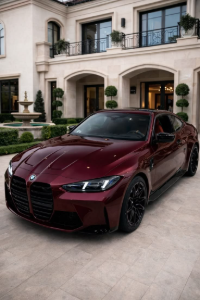
\includegraphics[width=\linewidth,height=4.1cm,keepaspectratio]{redimensionada.png}
\par\smallskip
{\footnotesize (a) Imagem de entrada}\par
\end{minipage}\hfill
\begin{minipage}[t]{.31\textwidth}
\centering
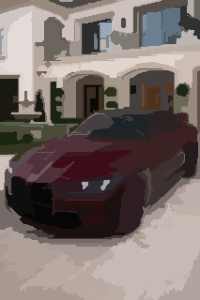
\includegraphics[width=\linewidth,height=4.1cm,keepaspectratio]{nivel_00.png}
\par\smallskip
{\footnotesize (b) Nível 1: 186 regiões}\par
\end{minipage}\hfill
\begin{minipage}[t]{.31\textwidth}
\centering

\includegraphics[width=\linewidth,height=4.1cm,keepaspectratio]{nivel_07.png}
\par\smallskip
{\footnotesize (c) Nível 8: 2 regiões}\par
\end{minipage}
\caption{Segmentação hierárquica da imagem do carro: entrada
redimensionada, nível inicial e nível mais agregado.}
\label{fig:visual}
\end{figure}

A primeira segmentação preserva variações locais de cor e contornos,
enquanto o oitavo nível resume a imagem em apenas duas regiões.
A redução do detalhamento é coerente com o aumento do MSE entre
732,3830 e 5.248,3535, conforme a Tabela~\ref{tab:hierarquia}.
O corte mais agregado não deve ser interpretado como detecção
semântica do veículo: as fusões dependem da adjacência espacial
e da diferença entre cores médias das regiões.

\subsection{Limitações}

O benchmark principal utiliza apenas
uma imagem e três resoluções.
Consequentemente, os resultados não
são suficientes para caracterizar
o desempenho em todas as classes
de imagens.

Também não foi realizada uma comparação
sistemática com outras implementações
de segmentação.

As medições dependem das condições
do ambiente computacional, embora
o procedimento tenha sido documentado
para permitir reprodução.

Por fim, a homogeneidade MSE não mede
diretamente a capacidade de reconhecer
objetos. A ausência de máscaras de
referência anotadas impede uma
avaliação quantitativa completa
da qualidade semântica.

Dessa forma, os resultados demonstram
o comportamento da implementação
e suas propriedades matemáticas,
mas não estabelecem superioridade
em relação a outros métodos.

% ============================================================
\subsection{Reprodutibilidade e ameaças à validade}

O script experimental registra os parâmetros, a revisão Git,
o hash SHA-256 da imagem e as versões do ambiente em um arquivo
JSON. Para cada resolução, há uma execução de aquecimento e cinco
repetições consecutivas. O arquivo de observações preserva os
tempos individuais; o resumo calcula média, desvio padrão amostral,
mediana, mínimo e máximo. Essas medidas permitem descrever a
variabilidade observada, mas não constituem intervalo de confiança.

A principal ameaça à validade externa é o uso de uma única imagem
natural no benchmark principal. A ampliação da resolução altera
simultaneamente o tamanho do grafo e a informação visual presente,
razão pela qual o MSE não deve ser comparado entre resoluções como
se fossem cortes de uma mesma partição. Além disso, os tempos
dependem do hardware, da carga do sistema e das versões das
bibliotecas, ainda que o procedimento possa ser reproduzido.

A avaliação utiliza o MSE para medir homogeneidade RGB, sem afirmar
que ele mede reconhecimento de objetos. O sistema implementa RI e VI,
mas a ausência de máscaras anotadas para a imagem de referência
impede uma avaliação quantitativa de acurácia semântica. Uma análise
mais abrangente exigiria imagens variadas, anotações humanas e
comparações controladas com métodos alternativos.

\section{Conclusão}
\label{sec:conclusao}
% ============================================================

Este trabalho apresentou a implementação
de uma ferramenta de segmentação hierárquica
de imagens baseada em grafos ponderados.

A solução utiliza estruturas próprias
de grafo e Union-Find, segmentação inicial
pelo método de Felzenszwalb--Huttenlocher,
agrupamento hierárquico de regiões e
visualização de grafos de adjacência.

A integração entre Python/FastAPI e React
permite configurar o processamento
e explorar diferentes níveis hierárquicos
de uma mesma imagem.

A avaliação matemática demonstrou
a preservação do aninhamento das partições
e a monotonicidade do MSE durante as fusões.

Os experimentos indicaram aumento
do custo computacional com a resolução,
com tempos médios entre 474,31 ms
e 3.257,31 ms nas configurações avaliadas.

Como trabalhos futuros, propõe-se ampliar
a variedade de imagens analisadas,
realizar comparações com métodos alternativos
e utilizar bases com segmentações de
referência para avaliação semântica.

% ============================================================
% REFERENCIAS
% ============================================================

\bibliographystyle{sbc}
\bibliography{referencias_grafos}

% LINK DO RELATÓRIO NO OVERLEAF
\section*{Disponibilidade do Projeto}
\par\smallskip

O código-fonte do relatório está disponível
na plataforma Overleaf:

\begin{center}
\url{https://www.overleaf.com/project/6b00a18a4f95ab59544f7e8e/share#7426e7e0d6b7d42f54da59cda79005dc6f9cf5927ce58da8}
\end{center}

\end{document}
